\documentclass[10pt,oneside,swedish]{lips}

%\usepackage[square]{natbib}\bibliographystyle{plainnat}\setcitestyle{numbers}
\usepackage[round]{natbib}\bibliographystyle{plainnat}

% Configure the document
\title{Generell mall}
\author{Redaktör namn}
\date{1 november 2016}
\version{1.0}

\reviewed{ReviewerName}{2015-xx-xx}
\approved{ApproverName}{2015-xx-xx}

\projecttitle{En inspirerande titel}

\groupname{Gruppnamn}
\groupemail{groupmail@liu.se}
\groupwww{http://www.isy.liu.se/tsrt10/group}

\coursecode{TSRT10}
\coursename{Reglerteknisk projektkurs}

\orderer{Beställare, Linköpings universitet}
\ordererphone{+46 xxxxxx}
\ordereremail{ordere@liu.se}

\customer{Kund, Företag X}
\customerphone{+46 xxxxxx}
\customeremail{customer@companyx.com}

\courseresponsible{Boss Person}
\courseresponsiblephone{+46 xxxxxx}
\courseresponsibleemail{the.boss@liu.se}

\supervisor{Handledare}
\supervisorphone{+46 xxxxxx}
\supervisoremail{super.visor@liu.se}

\smalllogo{logo} % Page header logo, filename
\biglogo{logo} % Front page logo, filename

\cfoot{\thepage}
\begin{document}
\maketitle

\cleardoublepage
\makeprojectid

\begin{center}
  \Large Projektdeltagare
\end{center}
\begin{center}
  \begin{tabular}{|l|l|l|}
    \hline
    \textbf{Namn} & \textbf{Ansvar} & \textbf{E-post}\\
    \hline
    Anna Andersson & kundansvarig (KUN) & Annan111@student.liu.se\\
    \hline
    Beata Bson & dokumentansvarig (DOK) & Beabs222@student.liu.se\\
    \hline
    Cecilia Cson & designansvarig (DES) & Ceccs333@student.liu.se\\
    \hline
    Doris Dson & testansvarig (TEST) & Dords444@student.liu.se\\
    \hline
    Erik Eson & kvalitetssamordnare (QA) & Eries555@student.liu.se\\
    \hline
    Fredrik Fson & implementationsansvarig (IMP) & Frefs666@student.liu.se\\
    \hline
    Greta Gson & Projektledare (PL) & Gregs777@student.liu.se\\
    \hline
  \end{tabular}
\end{center}


\cleardoublepage
\tableofcontents

\cleardoublepage
\section*{Dokumenthistorik}
\begin{tabular}{p{.06\textwidth}|p{.1\textwidth}|p{.45\textwidth}|p{.13\textwidth}|p{.13\textwidth}} 
  \multicolumn{1}{c}{\bfseries Version} & 
  \multicolumn{1}{|c}{\bfseries Datum} & 
  \multicolumn{1}{|c}{\bfseries Utförda förändringar} & 
  \multicolumn{1}{|c}{\bfseries Utförda av} & 
  \multicolumn{1}{|c}{\bfseries Granskad}\\
  \hline
  \hline
  0.1 & 2015-11-01 & Första utkast & Sign1 & Name1   \\
  \hline
  0.2 & 2015-11-03 & Första revision & Sign2 & Name2   \\
  \hline
\end{tabular}

\cleardoublepage
\pagenumbering{arabic}\cfoot{\thepage}

\section{Första kapitlet}
Detta är en text. \emph{Detta är kursiv text}. \textbf{Detta är text i
  fetstil}.


\subsection{Alternativ till dokumentmall}
Följande alternativ kan specificeras till dokumentmallen:
\begin{itemize}
\item Språk: \texttt{english} (default) eller \texttt{swedish}
\item Sidlayout: \texttt{oneside} (default) eller \texttt{twoside}
\item Fontstorlek: \texttt{10pt} (default), \texttt{11pt}, eller \texttt{12pt}
\end{itemize}
Exempel på mallaktivering
\begin{verbatim}
\documentclass[10pt,oneside,english]{lips}
\end{verbatim}
\subsection{Rubrik nivå 2}
\label{sec:rubrik-niva-2}
\lipsum[7]

\subsubsection{Rubrik nivå 3}
\label{sec:rubrik-niva-3}
\lipsum[7]

\subsection{Andra rubrik nivå 2}
\lipsum[7]

\subsection{Tredje rubrik nivå 2}
Mere text och en Laplace-transform av functionen $f(t)$
\begin{equation}
  F(s) = \int_{-\infty}^{\infty} f(t)e^{-st}\,dt.
\end{equation}

\section{Andra kapitlet}
Eulers identitet med $\pi$ är
\begin{equation}
  e^{i\pi} + 1 = 0
\end{equation}
och med $\tau$, se \citep{HartVi:2011} (se detta som ett exempel på
hur on-line resurser kan citeras), 
\begin{equation}
  e^{i\tau} = 1
\end{equation}
så här citeras ett vetenskapligt arbete\citep{einstein1905uber}, och
så här skrivs en fotnot\footnote{Var konsistent med hur ni citerar, i
  ingenjörsvetenskap så används fotnötter mycket
  sparsamt.}. Information om de citerade arbetena skrivs i filen \texttt{references.bib}.

\subsection{Ytterligare en rubrik på nivå 2}
\lipsum[10]

\begin{equation}
  \int_{a}^{b} f'(x)\,dx = f(b)-f(a)
\end{equation}

\section{Tredje kapitlet}
Matlab-kod kan infogas prydligt via paketet \texttt{listings.sty},
exempelvis så här\footnote{Här, koden från Matlab-kommandot
  \texttt{rank} används som exempel.}.
\begin{lstlisting}[language=Matlab,frame=single, numbers=left, stepnumber=2]
function r = rank(A,tol)
% RANK   Matrix rank.
%   RANK(A) provides an estimate of the number of linearly
%   independent rows or columns of a matrix A.
%   RANK(A,tol) is the number of singular values of A
%   that are larger than tol.
%   RANK(A) uses the default tol = max(size(A)) * eps(norm(A)).
%
%   Class support for input A:
%      float: double, single

%   Copyright 1984-2007 The MathWorks, Inc.

s = svd(A);
if nargin==1
   tol = max(size(A)) * eps(max(s));
end
r = sum(s > tol);
\end{lstlisting}

\subsection{Inkludera figurer}
\lipsum[7]

Figur~\ref{fig:bluemarble} vidsar en berömd bild på jorden från Apollo~17.
\begin{figure}[htbp]
  \centering
  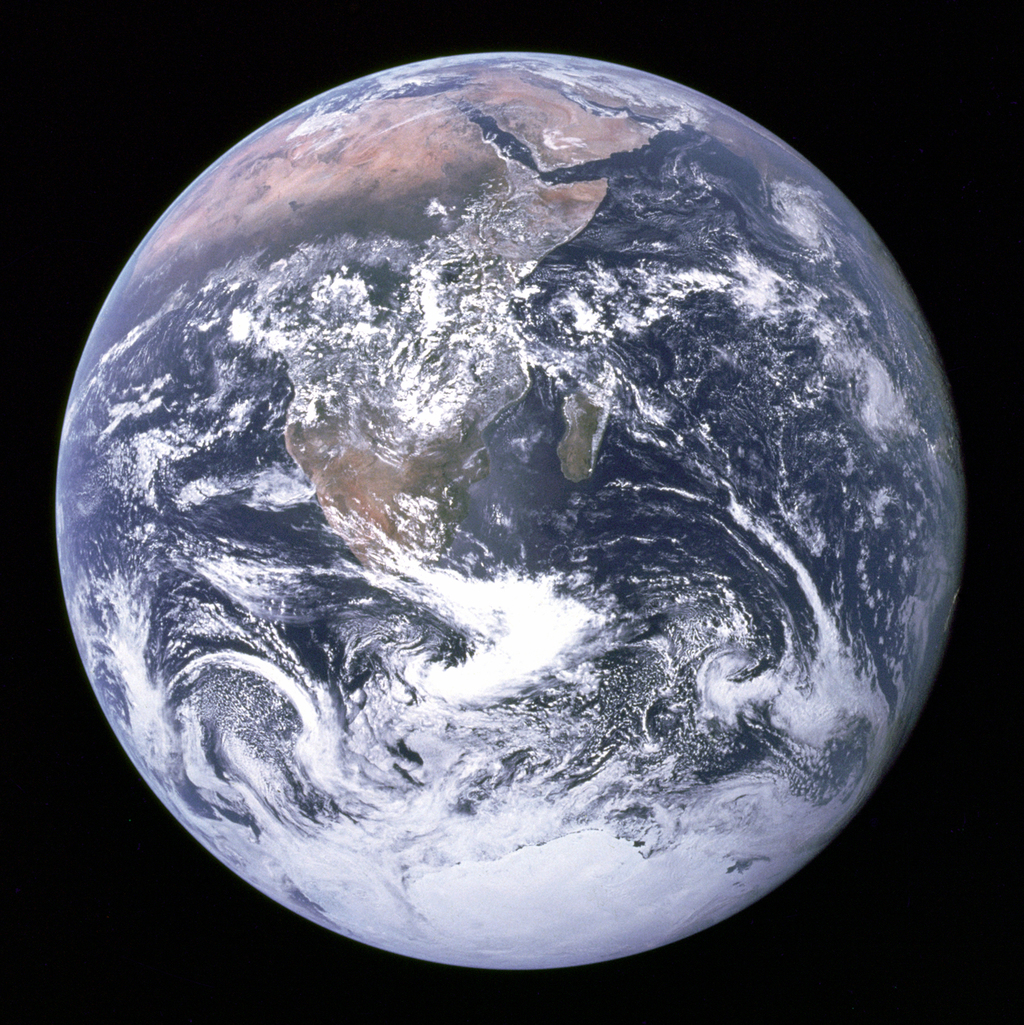
\includegraphics[width=.5\textwidth]{The_Earth_seen_from_Apollo_17}
  \caption{Det berömda 'The blue marble' fotot.}
  \label{fig:bluemarble}
\end{figure}

\section{\LaTeX{}}
Den här teten är ingen introduktion till \LaTeX{}. För mer
information, se online-resurser exempelvis på \citep{TUG}, där en bra
start är dokumentet \url{http://ctan.org/pkg/lshort}. Därifrån kan
även mjukvara for Linux
\url{http://www.tug.org/texlive/}, för Mac
\url{http://www.tug.org/mactex/}, och för Windows
\url{http://www.miktex.org} laddas ned.

För att typsätta det här dokumentet skriv
\begin{lstlisting}[language=sh,frame=single]
pdflatex general_sv.tex
bibtex general_sv
pdflatex general_sv.tex
\end{lstlisting}
vid en terminal prompt för att producera filen \texttt{lips-gen.pdf}.

\subsection{Att skriva krav}
\lipsum[7]

Det finns en miljö (environment) för att skriva krav, hantera
numrering, och göra det möjligt att referera individuella krav. Det
skall se bra ut även när tabellen spänner över flera sidor. Se
källkoden för tabellen med krav nedan.

\begin{requirements}
  \requirementno\label{req:myreq} & Description & 2\\
  \requirementno & Description & 1\\
  \requirementno & Description & 1\\
  \requirementno & Description & 1\\
  \requirementno & Description & 1\\
  \requirementno & Description & 1\\
  \requirementno & Description & 1\\
  \requirementno & Description & 1\\
  \requirementno & Description & 1\\
  \requirementno\label{req:myreq2} & Description & 2\\
  \requirementno & Description & 1\\
  \requirementno & Description & 1\\
  \requirementno & Description & 1\\
  \requirementno & Description & 1\\
  \requirementno & Description & 1\\
  \requirementno & Description & 1\\
  \requirementno & Description & 1\\
  \requirementno & Description & 1\\
  \requirementno & Description & 1\\
  \requirementno & Description & 1\\
  \requirementno & Description & 1\\
  \requirementno & Description & 1\\
  \requirementno & Description & 1\\
  \requirementno & Description & 1\\
  \requirementno & Description & 1\\
  \requirementno & Description & 1\\
  \requirementno & Description & 1\\
  \requirementno & Description & 1\\
  \requirementno & Description & 1\\
  \requirementno & Description & 1\\
\end{requirements}

Notera att kraven~\ref{req:myreq} och~\ref{req:myreq2} har prioritet 2.

\clearpage
\bibliography{references}

\cleardoublepage
\appendix
\section{Första appendix}
\subsection{Första underkapitel i första appendix}
\lipsum[5]

\subsubsection{Under underkapitel i första appendix}
En text.

\subsection{Andra underkapitel i första appendix}
\lipsum[5]
\subsubsection{Under underkapitel i första appendix}
En text

\section{Andra appendix}
\subsection{Första underkapitel i andra appendix}
\lipsum[5]

\subsubsection{Under underkapitel i andra appendix}
En text

\subsection{Andra underkapitel i andra appendix}
\lipsum[5]
\subsubsection{Under underkapitel i andra appendix}
En text

\end{document}

%%% Local Variables:
%%% mode: latex
%%% TeX-master: t
%%% End:
